\documentclass{beamer}

\usepackage{xltxtra}
\usepackage{graphicx}
%\usepackage[utf8]{inputenc}
\usepackage{fontspec}
\setmainfont{Verdana}
\setsansfont{Verdana}
\usepackage{tikz}
\usepackage{comment}
\usetikzlibrary{arrows,decorations.pathmorphing,backgrounds,fit,positioning,automata,calc,shapes.arrows,fadings}

\colorlet{mygray}{black!40}
\colorlet{mylightgray}{black!20}
\colorlet{mygreen}{green!60!black}
\definecolor{metroblue}{RGB}{0,59,126}
\definecolor{metroyellow}{RGB}{249,174,0}
\newcommand{\insertauthorpic}{
\includegraphics[width=1.446cm]{pics/philip.png}
\includegraphics[width=1.446cm]{pics/thomas.png}}
\newcommand{\footertext}{%
  \fontsize{5}{5}\selectfont\begin{minipage}{3mm}\vspace*{-1pt}\raggedleft\insertframenumber\end{minipage}\hspace*{3mm}
  © METRO AG.\hspace*{3mm}\insertshortauthor{}: \insertshorttitle{}
}
\newcommand{\datesize}{\fontsize{10}{10}\selectfont}
\newcommand{\metroslide}{%
{\setbeamercolor{background canvas}{bg=metroblue}
\begin{frame}[plain]
\centering

\includegraphics{pics/metro2.png}
\end{frame}
}
}



%TODO
\mode<presentation>
{
\setbeamerfont{block title}{size={}}
\usefonttheme{professionalfonts} % using non standard fonts for beamer
\usefonttheme{serif} % default family is serif
\setbeamercovered{transparent}
\setbeamertemplate{navigation bars}{}
\setbeamertemplate{navigation symbols}{}
\setbeamersize{text margin left=4mm}
\setbeamersize{text margin right=4mm}
\setbeamertemplate{itemize items}[ball]
\setbeamertemplate{enumerate items}[ball]
\setbeamertemplate{headline}{}
\setbeamertemplate{footline}{
  \begin{tikzpicture}[remember picture,overlay]
  \draw[metroblue] ($(current page.south west)+(0.6,0.6)$) -- ($(current page.south east)+(-3.5,0.6)$);
  \node (logosmall) at ($(current page.south east)+(-0.2,-0.1)$) [anchor=south east] {
\includegraphics[height=8mm]{metro.png}};
  \node[metroblue] (textline) at ($(current page.south west)+(0.8,0.13)$) [anchor=south west] {\footertext{}};
  \end{tikzpicture}
}
\defbeamertemplate*{title page}{metro}[1][]{
  \begin{tikzpicture}[remember picture,overlay]
  \node (logo) at (current page.north west) [anchor=north west] {
\includegraphics[height=\paperheight]{left.png}};
  \node[white] (title) at ($(logo)+(-0.7,0.65)$) [anchor=south west] {\fontsize{20}{20}\selectfont\textbf{\inserttitle}\par};
  \node[white] (subtitle) [below=0.7 of title.west,anchor=west] {\fontsize{12}{12}\selectfont\textbf{\insertsubtitle}\par};
  \node[white] (date) [below=0.9 of subtitle.west,anchor=west] {\datesize\insertdate,};
  \node[white] (place) [below=0.42 of date.west,anchor=west] {\datesize\selectfont\location};
  \node[white] (authorpic) [below=0.1 of place.south west,anchor=north west] {\insertauthorpic};
  \node[white] (author) [right=0.1 of authorpic.south east,anchor=south west] {\datesize\selectfont\insertauthor};
  \node[white] (textline) at ($(current page.south west)+(0.8,0.13)$) [anchor=south west] {\footertext{}};
  \end{tikzpicture}
}
\defbeamertemplate*{frametitle}{metro}[1][]{
  \vskip2mm%
  \hspace*{3mm}\fontsize{16}{12}\selectfont\textbf{\textcolor{metroblue}{\insertframetitle}}
}
}


\begin{document}

\title[React and Reflux]{REACT AND REFLUX:}
\subtitle{Components, Actions, Stores, and State}
\author[P.\ Baues, T.\ Str\"oder]{Philip Baues and Thomas Str\"oder}
\date{28./29.\ September 2017}
\newcommand{\location}{\texttt{code.talks} Hamburg}

{\setbeamercolor{background canvas}{bg=metroblue}
\begin{frame}[plain]
\centering

\includegraphics{metro2.png}
\end{frame}
}

{\setbeamercolor{background canvas}{bg=metroblue}
\begin{frame}[plain]
\titlepage
\end{frame}
}

\begin{comment}
Abstract:
React is currently one of the most popular ingredients of modern web applications. It is a component-based JavaScript library supporting the decomposition of big web applications into small parts, especially following principles like single responsibility and separation of concerns. However, on its own it lacks concise support for transversal state handling when parts of an application should alter the state of another part and these parts are not in a father-child-like relationship. To this end, the Reflux JavaScript library adds actions and stores for state handling.

In this talk, we will have a look at general patterns how to use React components together with Reflux stores and actions to build a responsive web application. Here, the focus is on state: When and where to (not) have it and how to deal with it using the facilities React and Reflux are offering. We illustrate these concepts with a small web shop example. In addition to that, we also address common mistakes and how to avoid them.
\end{comment}

\begin{frame}\frametitle{Why React?}
\centering
\begin{tikzpicture}
\node[anchor=north west] (text1) at (0,6.1) {declarative view abstraction};
\fill[draw=metroblue,fill=metroblue!50,rounded corners=10] (6,0) rectangle (10,3);
\node[anchor=north west] at (6.1,2.9) {Component};
\fill[draw=metroyellow,fill=metroyellow!50,rounded corners=10] (6.9,0.1) rectangle (9.9,2.1);
\node[anchor=north west] at (7,2) {\small Component};
\fill[draw=metroblue,fill=metroblue!50,rounded corners=10] (6,3.1) rectangle (10,6.1);
\node[anchor=north west] at (6.1,6) {Component};
\node (text2) [below=of text1.west, anchor=west] {decoupling};
\node (text3) [below=of text2.west, anchor=west] {easy testing};
\node (text4) [below=of text3.west, anchor=west] {fast rendering};
\end{tikzpicture}
\end{frame}

\begin{frame}\frametitle{React Components}
\centering
\tikzfading[name=fade left,
right color=transparent!0,
left color=transparent!100]
\begin{tikzpicture}
\node (component) {Component};
\visible<3->{\node (proparrow) [above left=0.1 of component,single arrow,shape border uses incircle,
shape border rotate=315,fill=metroblue,minimum height=2cm,path fading=fade left,fading transform={rotate=315}] {};}
\visible<3->{\node [above left=0.1 of proparrow] {\phantom{t}props};}
\visible<5->{\node (statearrow) [above right=0.1 of component,double arrow,shape border uses incircle,
shape border rotate=225,fill=red,minimum height=2cm] {};}
\visible<5->{\node [above right=0.1 of statearrow] {state\phantom{p}};}
\visible<2->{\node (renderarrow) [below=0.1 of component,single arrow,shape border uses incircle,
shape border rotate=270,fill=mygreen,minimum height=2cm,path fading=fade left,fading transform={rotate=270}] {};}
\visible<2->{\node [below=0.1 of renderarrow] {rendering};}
\visible<4->{\node (lifearrow) [above=0.1 of component,double arrow,shape border uses incircle,shape border rotate=90,
fill=red,minimum height=2cm] {};}
\visible<4->{\node [above=0.1 of lifearrow] {lifecycle};}
\end{tikzpicture}
\end{frame}

\begin{frame}\frametitle{React Components \textendash{} Example}
\centering
Code!
\end{frame}

\begin{frame}\frametitle{Components}
\centering
\tikzfading[name=fade left,
right color=transparent!0,
left color=transparent!100]
\begin{tikzpicture}
\node (component) {Component};
\node (proparrow) [above left=0.1 of component,single arrow,shape border uses incircle,
shape border rotate=315,fill=metroblue,minimum height=2cm,path fading=fade left,fading transform={rotate=315}] {};
\node [above left=0.1 of proparrow] {\phantom{t}props};
\visible<3->{\node (statearrow) [above right=0.1 of component,single arrow,shape border uses incircle,
shape border rotate=225,fill=red,minimum height=2cm,path fading=fade left,fading transform={rotate=225}] {};}
\visible<-2>{\node (statearrow2) [above right=0.1 of component,double arrow,shape border uses incircle,
shape border rotate=225,fill=red,minimum height=2cm] {};}
\node [above right=0.1 of statearrow] {state\phantom{p}};
\node (renderarrow) [below=0.1 of component,single arrow,shape border uses incircle,
shape border rotate=270,fill=mygreen,minimum height=2cm,path fading=fade left,fading transform={rotate=270}] {};
\node [below=0.1 of renderarrow] {rendering};
\visible<-1>{\node (lifearrow) [above=0.1 of component,double arrow,shape border uses incircle,shape border rotate=90,
fill=red,minimum height=2cm] {};}
\visible<-1>{\node [above=0.1 of lifearrow] {lifecycle};}
\end{tikzpicture}
\end{frame}

\begin{frame}\frametitle{Why Reflux?}
\centering
\begin{tikzpicture}
\node[anchor=north west] (text1) at (0,6.1) {declarative view abstraction};
\fill[draw=metroblue,fill=metroblue!50,rounded corners=10] (6,0) rectangle (10,3);
\node[anchor=north west] at (6.1,2.9) {Component};
\fill[draw=metroyellow,fill=metroyellow!50,rounded corners=10] (6.9,0.1) rectangle (9.9,2.1);
\node[anchor=north west] at (7,2) {\small Component};
\fill[draw=metroblue,fill=metroblue!50,rounded corners=10] (6,3.1) rectangle (10,6.1);
\node[anchor=north west] at (6.1,6) {Component};
\fill[draw=red,fill=red!50,rounded corners=10] (3.5,3.1) rectangle (5.5,5.1);
\node[anchor=north west] at (3.6,5) {Store};
\node (text2) [below=of text1.west, anchor=west] {\textcolor{red}{decoupling}};
\node (text3) [below=of text2.west, anchor=west] {\textcolor{red}{easy testing}};
\node (text4) [below=of text3.west, anchor=west] {fast rendering};
\node (text5) [below=of text4.west, anchor=west] {\textcolor{red}{transversal state handling}};
\draw (5.5,4.1) edge[<->,red,thick] (6,4.1);
\draw (5.4,3.2) edge[<->,red,thick] (6.1,2.9);
\end{tikzpicture}
\end{frame}

\begin{frame}\frametitle{Data Flow}
\centering
\begin{tikzpicture}
[node/.style={rectangle,draw=black,thick,inner sep=5pt},
edge/.style={->,thick},
connect/.style={->,thick,dashed}]
\node[node] (action) {Action};
\node[node] (component) [below left=2 of action] {Component};
\node[node] (store) [below right=2 of action] {Store};
\draw (component) edge[edge,in=180,out=90] node[auto] {calls} (action);
\draw (action) edge[edge,in=90,out=0] node[auto] {executes} (store);
\draw (store) edge[edge,in=270,out=270] node[auto] {sets state} (component);
\draw (component) edge[connect,bend right=30] node[auto,swap] {sets store(s)} (store);
\draw (store) edge[connect,in=270,out=180] node[auto] {listens to} (action);
\end{tikzpicture}
\end{frame}

\begin{comment}
Notes on Reflux components:
* Set multiple stores by setting this.stores (the plural) and setting it to an Array of store classes.
* Set a this.storeKeys Array to restrict only certain parts of the store being mixed into the component state.
\end{comment}
\begin{frame}\frametitle{Reflux Components}
\centering
\tikzfading[name=fade left,
right color=transparent!0,
left color=transparent!100]
\begin{tikzpicture}
\node (component) {Component};
\node (proparrow) [above left=0.1 of component,single arrow,shape border uses incircle,
shape border rotate=315,fill=metroblue,minimum height=2cm,path fading=fade left,fading transform={rotate=315}] {};
\node [above left=0.1 of proparrow] {\phantom{t}props};
\node (statearrow) [above right=0.1 of component,single arrow,shape border uses incircle,
shape border rotate=225,fill=red,minimum height=2cm,path fading=fade left,fading transform={rotate=225}] {};
\node [above right=0.1 of statearrow] {state\phantom{p}};
\node (renderarrow) [below=0.1 of component,single arrow,shape border uses incircle,
shape border rotate=270,fill=mygreen,minimum height=2cm,path fading=fade left,fading transform={rotate=270}] {};
\node [below=0.1 of renderarrow] {rendering};
\node [above=2.5 of component] {extend React components};
\node [below left=0.5 of component] {\begin{minipage}{3cm}\begin{center}only\\interaction\\logic\end{center}\end{minipage}};
\node [below right=0.5 of component] {\begin{minipage}{3cm}\begin{center}treat state as\\read-only\end{center}\end{minipage}};
\end{tikzpicture}
\end{frame}

\begin{frame}\frametitle{Actions}
\centering
\begin{tikzpicture}
\node (action) {Action};
\visible<2->{\node [above=of action] {just a function};}
\visible<3->{\node (callarrow) [below left=0.1 of action,single arrow,shape border uses incircle,
shape border rotate=45,fill=metroblue,minimum height=2cm,path fading=fade left,fading transform={rotate=45}] {};}
\visible<3->{\node [below left=0.1 of callarrow] {\begin{minipage}{3cm}\begin{center}called by component\end{center}\end{minipage}};}
\visible<4->{\node (transarrow) [below right=0.1 of action,single arrow,shape border uses incircle,
shape border rotate=315,fill=mygreen,minimum height=2cm,path fading=fade left,fading transform={rotate=315}] {};}
\visible<4->{\node [below right=0.1 of transarrow] {\begin{minipage}{3cm}\begin{center}transports payload\end{center}\end{minipage}};}
\end{tikzpicture}
\end{frame}

\begin{frame}\frametitle{Stores}
\centering
\begin{tikzpicture}
\node (store) {Store};
\visible<2->{\node [above=of store] {state handler};}
\visible<3->{\node (listenarrow) [below left=0.1 of store,single arrow,shape border uses incircle,
shape border rotate=45,fill=metroblue,minimum height=2cm,path fading=fade left,fading transform={rotate=45}] {};}
\visible<3->{\node [below left=0.1 of listenarrow] {\begin{minipage}{3cm}\begin{center}listens to actions\end{center}\end{minipage}};}
\visible<4->{\node (setarrow) [below right=0.1 of store,single arrow,shape border uses incircle,
shape border rotate=315,fill=mygreen,minimum height=2cm,path fading=fade left,fading transform={rotate=315}] {};}
\visible<4->{\node [below right=0.1 of setarrow] {\begin{minipage}{3cm}\begin{center}sets state of components\end{center}\end{minipage}};}
\visible<5->{\node [below=2.5 of store] {only data logic};}
\end{tikzpicture}
\end{frame}

\begin{frame}\frametitle{Reflux Components, Actions, and Stores \textendash{} Example}
\centering
Code!
\end{frame}

\begin{frame}\frametitle{Introduction}
\centering
\begin{itemize}
\item Historically grown company and IT-systems
\item Digital readiness initiative to renew whole IT landscape
\item \textit{Betty} as first customer journey and system
\item A lot of different other applications in development\\
(Driver App, sales and more, customer master data, …)
\end{itemize}
\end{frame}

\begin{frame}\frametitle{What is Betty}
\centering
\begin{center}
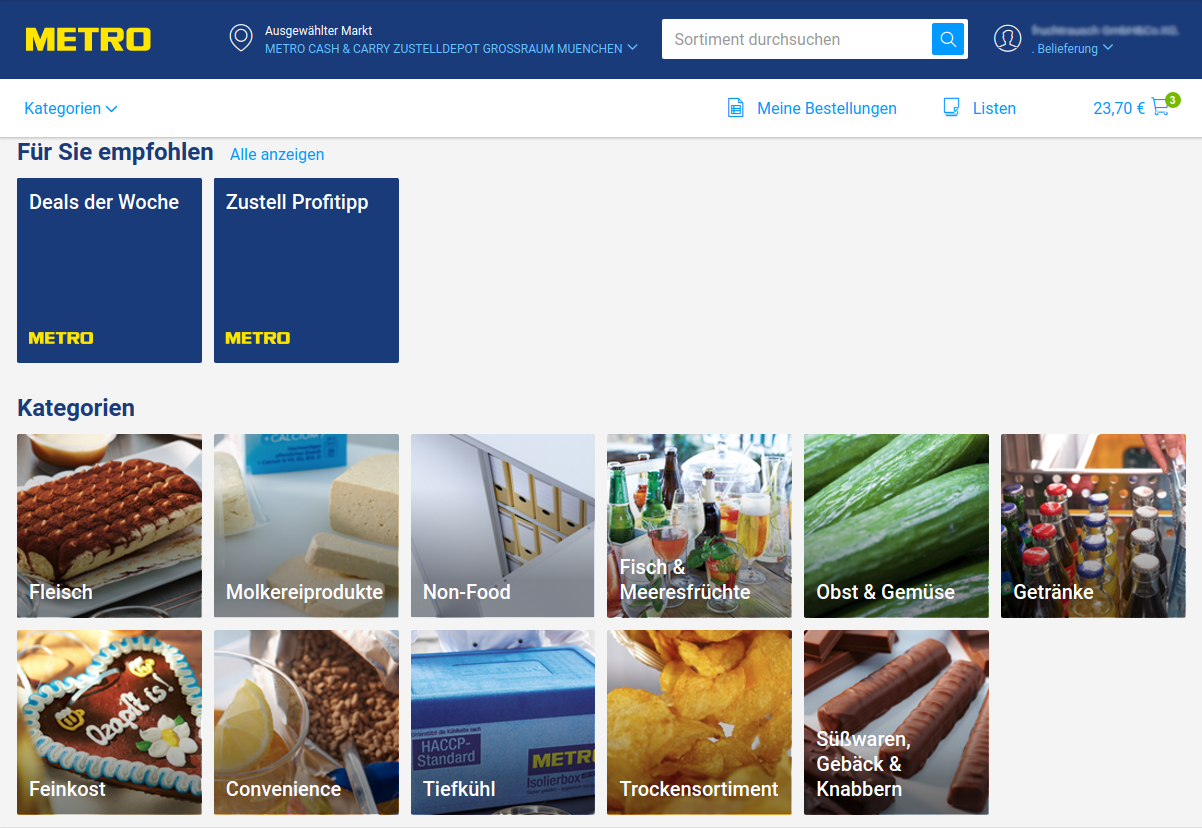
\includegraphics[width=.85\linewidth,height=.85\textheight,keepaspectratio]{Betty.png}
\end{center}
\end{frame}

\end{document}

